\documentclass[11pt]{article}

% ---------------------------------------------------------------------------
% Packages
% ---------------------------------------------------------------------------
\usepackage[utf8]{inputenc}
\usepackage[greek,english]{babel}   % english is the MAIN language (report is in English)
\usepackage[a4paper,margin=2.5cm]{geometry}
\usepackage{graphicx}
\usepackage{amsmath,amssymb}
\usepackage{xcolor}
\usepackage{booktabs}
\usepackage{caption}
\usepackage{enumitem}
\usepackage{float}
\usepackage{listings}
\usepackage{tcolorbox}
\usepackage[colorlinks=true,linkcolor=blue,citecolor=blue,urlcolor=blue]{hyperref}

\usepackage{tikz}
\usetikzlibrary{shapes.geometric, arrows, positioning, fit}

% Define block styles
\tikzstyle{block} = [rectangle, draw, fill=blue!10, text width=5em, text centered, minimum height=3em]
\tikzstyle{arrow} = [thick,->,>=stealth]

% all figures are kept self-contained in the report assets folder
\graphicspath{{rs1_report_assets/}}

% ---------------------------------------------------------------------------
% EDIT ME: the public page hosting the robot videos
% ---------------------------------------------------------------------------
\newcommand{\videourl}{https://github.com/mk4ll/Biped-Locomotion-Challenge}

\title{
    \vspace*{-2.5cm}
    
\includegraphics[width=10cm]{up_2017_logo_gr.png}\\[0.4em]
    Department of Electrical \& Computer Engineering\\[0.4em]
    Robotic Systems I (ECE\_DK808) \\[0.3em]
    Project 5: Biped Locomotion Challenge - Simulation, Walking Control
}
\author{Kalloniatis Ilias Marios\\Student ID: 1100879\\up1100879@ac.upatras.gr
        \and Kanellopoulos Konstantinos\\Student ID: 1100881\\up1100881@ac.upatras.gr}
\date{Academic Year: 2025--26}

\begin{document}
\selectlanguage{english}

\maketitle
\thispagestyle{empty}

% ---------------------------------------------------------------------------
% Video / code box (before the abstract)
% ---------------------------------------------------------------------------
\begin{center}
\begin{tcolorbox}[colback=blue!4,colframe=blue!55!black,width=0.92\textwidth,
    arc=3pt,boxrule=1pt,left=10pt,right=10pt,top=8pt,bottom=8pt]
\centering
\textbf{\large Demonstration videos \& source code}\\[4pt]
The robot videos (flat / incline / stairs walking, push recovery, omnidirectional
walking, and the extended demonstrations) together with the full source code are
available at:\\[6pt]
{\large \href{\videourl}{\videourl}}
\end{tcolorbox}
\end{center}

\vspace{0.5em}

% ---------------------------------------------------------------------------
% Abstract
% ---------------------------------------------------------------------------
\begin{abstract}
\noindent
We present a dynamics-first, torque-level walking controller for two humanoid
robots - the \textbf{Unitree~G1} (33~kg, 29~DoF) and the \textbf{PAL~Talos}
(94~kg, 32~DoF) - in the MuJoCo simulator. At every control step a
\emph{whole-body Quadratic Program (QP) inverse-dynamics} problem is solved and
\emph{joint torques} are commanded, rather than tracking kinematic references
with position servos. The controller is organised as a clean
\mbox{offline~$\rightarrow$~online~$\rightarrow$~whole-body-control} pipeline: an
offline layer plans footsteps and a Zero-Moment-Point reference; an online layer
closes the loop on the \emph{Divergent Component of Motion} (DCM / capture point)
and reactively adjusts foot placement; and the QP realises the resulting Centre-of-Mass,
swing-foot, torso and posture tasks subject to the floating-base dynamics,
surface-frame friction cones and torque limits. Expressing all balance quantities
with respect to gravity and the local contact surface lets the same controller
generalise from flat ground to inclines and small stairs without redesign. The
system achieves continuous flat walking, single-support balancing, weight shifting,
push recovery, omnidirectional walking (forward / backward / strafing / turning),
uphill walking up to $16^{\circ}$, and stair climbing; a simple slip-versus-tip
analysis predicts the static standing limit ($\approx\!27^{\circ}$, i.e.
$\arctan\mu$), which the experiments confirm. The robot-agnostic design runs every
task on both robots. We additionally showcase two integrated demonstrations of
path planning and disturbance handling: a ``waiter'' that weaves a slalom around
randomly generated tables while keeping a tray level, and a ``Sisyphus'' that
pushes a boulder up a slope.
\end{abstract}

% ---------------------------------------------------------------------------
% Table of contents on its own page
% ---------------------------------------------------------------------------
\newpage
\tableofcontents
\newpage

% ===========================================================================
\section{Introduction}
\label{sec:intro}

Bipedal locomotion is a canonical underactuated control problem: a humanoid is
supported only through unilateral, friction-limited contacts and must continuously
move its centre of mass (CoM) over the supporting foot to step without falling.
This project (\emph{Biped Locomotion Challenge}) targets a
\emph{simulation-only} walking controller for a humanoid in MuJoCo, focusing on
balance maintenance, weight shifting, and stable double-support~$\leftrightarrow$~single-support
transitions.

\paragraph{Objectives (assignment core tasks).}
\begin{enumerate}[label=(\alph*),itemsep=2pt]
    \item generate stable, continuous walking;
    \item plan and control CoM trajectories for stable locomotion;
    \item shift the body weight to stabilise over the support foot in single support;
    \item coordinate foot placement and body motion for continuous stepping;
    \item maintain stability through support-phase transitions;
    \item recover from small disturbances and imperfect foot placement.
\end{enumerate}

\paragraph{Approach and contributions.}
We adopt a \emph{dynamics-first} design: a per-step whole-body QP inverse-dynamics
controller that outputs joint torques, driven by a DCM-based planning/feedback
layer. Our main contributions are:
\begin{itemize}[itemsep=2pt]
    \item a torque-level whole-body QP with hard floating-base dynamics and
          \emph{surface-frame} friction cones, with a safe fallback when infeasible;
    \item a DCM (capture-point) planning and feedback layer with reactive step
          adjustment for push recovery;
    \item a \emph{terrain-aware} formulation that generalises to inclines and small
          stairs, plus a short slip-vs-tip analysis of the standing limit;
    \item a \emph{robot-agnostic} stack that runs identically on the G1 and Talos;
    \item omnidirectional walking and two integrated path-planning demonstrations.
\end{itemize}

% ===========================================================================
\section{Theoretical Background}
\label{sec:theory}

\subsection{Floating-base dynamics}
With generalised coordinates $q$ and velocities $v$ (the first 6 DoF being the
unactuated floating base), the rigid-body dynamics in contact are
\begin{equation}
    M(q)\,\dot v + h(q,v) \;=\; S^{\top}\tau \;+\; \textstyle\sum_c J_c^{\top} f_c ,
    \label{eq:dyn}
\end{equation}
where $M$ is the mass matrix, $h$ the bias (Coriolis, centrifugal and gravity)
term, $S$ the actuation selection matrix, and $J_c,\,f_c$ the contact Jacobian
and force at each contact point.

\subsection{Whole-body control as a QP}
Tasks are imposed at the acceleration level, $a_{\mathrm{des}} = a_{\mathrm{ref}}
+ K_p e + K_d \dot e$, giving residuals $J_i\dot v - b_i$. With decision variables
$x=[\dot v;\,\tau;\,f]$ we solve
\begin{equation}
    \min_{x}\; \sum_i w_i \lVert J_i\dot v - b_i\rVert^2
    \;\; \text{s.t.}\;\;
    \text{Eq.~\eqref{eq:dyn}},\;\; J_c\dot v + \dot J_c v = 0,\;\;
    \text{friction cones},\;\; \tau_{\min}\!\le\!\tau\!\le\!\tau_{\max}.
    \label{eq:wbc}
\end{equation}

\subsection{LIPM, ZMP and the Divergent Component of Motion (DCM)}
Under the Linear Inverted Pendulum Model the Zero-Moment Point satisfies
$p_{\mathrm{zmp}} = x_{\mathrm{com}} - (z/g)\,\ddot x_{\mathrm{com}}$. Defining the
DCM (capture point) $\xi = x + \dot x/\omega$ with $\omega=\sqrt{g/z}$ splits the
CoM dynamics into a stable part and the single unstable mode
\begin{equation}
    \dot\xi = \omega\,(\xi - p_{\mathrm{zmp}}),
    \label{eq:dcm}
\end{equation}
which yields a clean feedback law and makes ``where to step not to fall''
$\approx$ ``step toward the DCM''.

\subsection{Friction cones and the incline}
Each contact force must lie in its linearised friction cone, expressed in the
\emph{surface} frame (normal $n=$ surface normal, not world-$z$):
$f_n\ge f_{\min},\; |f_{t_1}|\le\mu f_n,\; |f_{t_2}|\le\mu f_n$. On a slope of angle
$\alpha$, a static body \emph{slips} when $\tan\alpha>\mu$ and \emph{tips} when the
gravity line leaves the support; we use this in Sec.~\ref{sec:incline}.

% ===========================================================================
\section{System Architecture}
\label{sec:arch}

The controller is a three-stage pipeline: an
\textbf{offline} layer (footstep planner, ZMP reference, backward-recursion DCM
trajectory, swing-foot splines, gait FSM); an \textbf{online} layer (DCM feedback,
capture-point step adjustment, terrain-aware friction orientation, CoM-height
regulation, heading); and the \textbf{whole-body QP} \eqref{eq:wbc} that outputs
torques to MuJoCo, with state feedback closing the loop.

\begin{figure}[H]
\centering
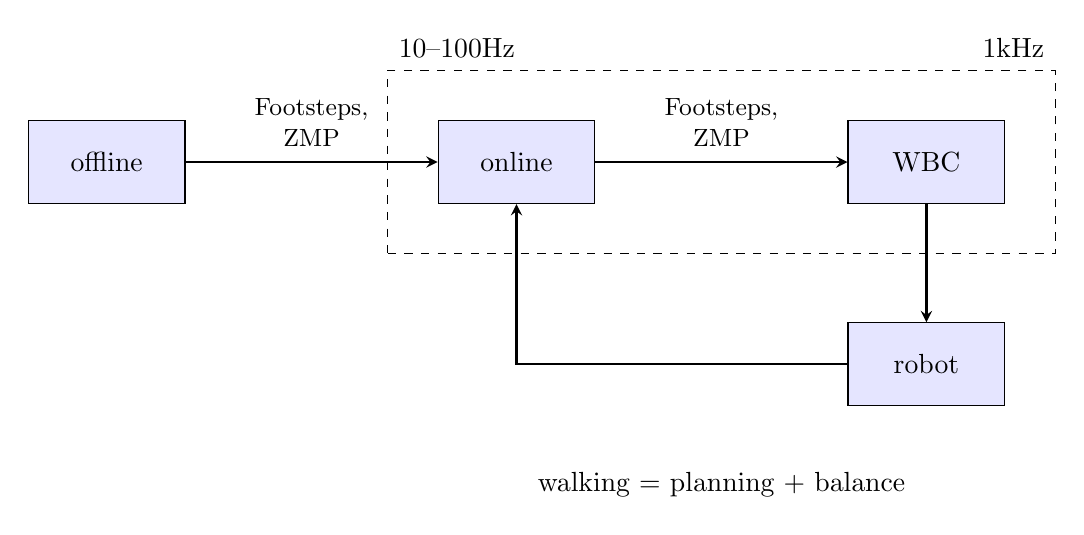
\begin{tikzpicture}[
    % Setting up styles here keeps the drawing code clean
    block/.style = {rectangle, draw, fill=blue!10, text width=5em, text centered, minimum height=3em},
    arrow/.style = {thick, ->, >=stealth},
    lbl/.style = {midway, above, align=center, font=\small, yshift=2pt}
]

    % 1. Place nodes with exact horizontal/vertical gaps (border-to-border)
    \node (offline) [block] {offline};
    \node (online)  [block, right=3.2cm of offline] {online};
    \node (wbc)     [block, right=3.2cm of online] {WBC};
    
    % Robot node directly below WBC
    \node (robot)   [block, below=1.5cm of wbc] {robot};

    % 2. Dashed box wrapping online and WBC with comfortable padding (inner sep)
    \node (innerloop) [draw, dashed, inner sep=18pt, fit=(online) (wbc)] {};

    % 3. Frequencies positioned precisely on top of the dashed box corners
    \node[anchor=south west, inner sep=4pt] at (innerloop.north west) {10--100Hz};
    \node[anchor=south east, inner sep=4pt] at (innerloop.north east) {1kHz};
    
    % 4. Arrows with line-broken text to save horizontal space and prevent overlap
    \draw [arrow] (offline) -- (online) node[lbl] {Footsteps,\\ ZMP};
    \draw [arrow] (online)  -- (wbc)    node[lbl] {Footsteps,\\ ZMP};
    
    % 5. Feedback loops
    \draw [arrow] (wbc) -- (robot);
    \draw [arrow] (robot.west) -| (online.south);

    % 6. Equation placed neatly below the entire structure, vertically aligned with the robot
    \node at ([yshift=-1cm]innerloop.south |- robot.south) {walking = planning + balance};

\end{tikzpicture}
\caption{System architecture and control loops}
\label{fig:architecture}
\end{figure}

% ===========================================================================
\section{Implementation}
\label{sec:impl}
The controller is implemented in Python on MuJoCo~3.4. The code is organised by
the pipeline of Sec.~\ref{sec:arch}: \texttt{src/sim} (model loading and a thin
environment wrapper), \texttt{src/dynamics} (model terms and contacts),
\texttt{src/control} (the whole-body QP, tasks, and the walking controller), and
\texttt{src/planning} (footsteps, FSM, DCM, swing trajectories, terrain). A single
\texttt{config/params.yaml} holds every gain, weight and timing; nothing is
hard-coded. The QP is solved with \texttt{quadprog} (a dense, strictly convex
solver) and falls back to \texttt{clarabel}/\texttt{osqp} if a step is infeasible.

\subsection{Robot models and torque actuators}
\label{sec:impl:models}
Both robots are loaded from the MuJoCo Menagerie. The G1 ships with \emph{position}
servos, so at load time we rewrite all 29 actuators to \emph{motor} (torque)
actuators and re-apply each joint's torque limit (e.g.\ $\pm88$~N\,m at the hips,
$\pm139$~N\,m at the knees), since motors do not inherit \texttt{actuatorfrcrange}.
We add four contact-corner sites under each foot (used as the contact points for
the friction cones). The PAL Talos (\texttt{scene\_motor.xml}) already ships torque
motors but uses \emph{box} feet, so we inject the four corner sites onto the foot
box via \texttt{mjSpec} at load time. A single \texttt{RobotConfig}
(\texttt{src/sim/robots.py}) captures everything that differs between the two
robots --- base/torso bodies, foot sites and corners, the bent-knee crouch pose,
and the ankle joints --- making the entire controller \emph{robot-agnostic}: the
same code runs the 33~kg G1 and the 94~kg Talos. Both start from a statically
balanced \emph{bent-knee crouch} (feet flat, CoM lowered to $\approx\!0.65$~m for
the G1) so that walking shows naturally flexed knees; the arms are parked in a
fixed posture and held by the posture task.

\subsection{Dynamics terms}
\label{sec:impl:dyn}
Per control step, \texttt{ModelTerms} extracts the quantities of
Eq.~\eqref{eq:dyn}: the mass matrix $M$ via \texttt{mj\_fullM}, the bias $h$ via
\texttt{data.qfrc\_bias} (which already contains Coriolis, centrifugal and gravity
terms), the selection matrix $S$, the translational contact Jacobians of the foot
corners (\texttt{mj\_jacSite}), and a 6-D Jacobian at each foot site for the rigid
contact constraint. The convective term $\dot J\,v$ is obtained from the spatial
site acceleration with $\ddot q\!=\!0$; crucially we \emph{also} zero gravity while
computing it, because MuJoCo's \texttt{mj\_objectAcceleration} otherwise folds the
gravitational offset into the acceleration and corrupts $\dot J v$ --- a subtle bug
that, before being fixed, made the QP believe the robot was in free fall.

\subsection{Whole-body QP and tasks}
\label{sec:impl:wbc}
The QP \eqref{eq:wbc} uses decision variables $x=[\dot v;\,\tau;\,f]$. The
floating-base dynamics \eqref{eq:dyn} enter as a hard equality. A rigid foot would
make the four corner constraints redundant (12 scalar equations for a 6-DoF foot),
which the solver flags as infeasible; we therefore impose the
\emph{non-acceleration} constraint once, as a \emph{6-D constraint at the foot
site} (full rank), while keeping a 3-D force per corner for the friction
pyramid and centre-of-pressure. Friction cones are built in the \emph{surface
frame} via a rotation $R_{\text{surf}}$ (identity on flat ground, the slope
rotation on an incline), and torque limits enter as bounds. The cost stacks the
weighted task residuals (Table~\ref{tab:params}): a high-weight \textbf{CoM} task,
a \textbf{torso/pelvis orientation} task that keeps the trunk vertical
\emph{with respect to gravity}, a low-weight \textbf{posture} regularisation toward
the crouch, and a \textbf{swing-foot} task that is active only while a foot is
airborne. The CoM command itself is not a plain position PD: in the horizontal
plane it is the DCM feedback law derived from \eqref{eq:dcm}
($\dot\xi_{\text{cmd}}=\dot\xi_{\text{ref}}+k(\xi_{\text{ref}}-\xi)$, then
$p_{\text{zmp}}^{\text{cmd}}=\xi-\dot\xi_{\text{cmd}}/\omega$ and
$a_{\text{com}}=\omega^2(x-p_{\text{zmp}}^{\text{cmd}})$), while the vertical axis
tracks a low-passed CoM height. Joint torques are read directly from the QP
solution and sent to MuJoCo.

\subsection{Planning: footsteps, FSM, DCM, swing}
\label{sec:impl:plan}
The offline layer (\texttt{src/planning}) produces a continuous reference. The
\textbf{footstep planner} places alternating left/right steps from a desired step
length (or a body-frame velocity command, or an arbitrary 2-D path), with a
kinematic clamp. The \textbf{gait FSM} builds the phase timeline
$\text{DS}_{\text{init}}\!\to\!\text{SS}\!\to\!\text{DS}\!\to\!\dots$ with the
support/swing assignment and the per-phase ZMP endpoints. The \textbf{DCM planner}
fixes the ZMP at the stance foot during single support and integrates
\eqref{eq:dcm} \emph{backward} (the stable direction) from a terminal condition
$\xi_{\text{end}}=p_{\text{zmp,end}}$, then integrates the CoM \emph{forward}; this
keeps the ZMP inside the support polygon by construction. The \textbf{swing planner}
uses a smoothstep in the horizontal plane and a $(1-\cos)$ vertical bump (zero foot
velocity at lift-off, apex and touchdown for a soft landing). An online
\textbf{capture-point} adjustment shifts the swing-foot target by
$k(\xi_{\text{meas}}-\xi_{\text{ref}})$, updated throughout the step, which is what
provides push recovery (Sec.~\ref{sec:results}). The planner outputs are sampled by
the controller as $\texttt{reference}(t)$ and are completely independent of the
robot --- Fig.~\ref{fig:plan} shows the offline plan alone, before any robot moves.

\begin{figure}[H]\centering
  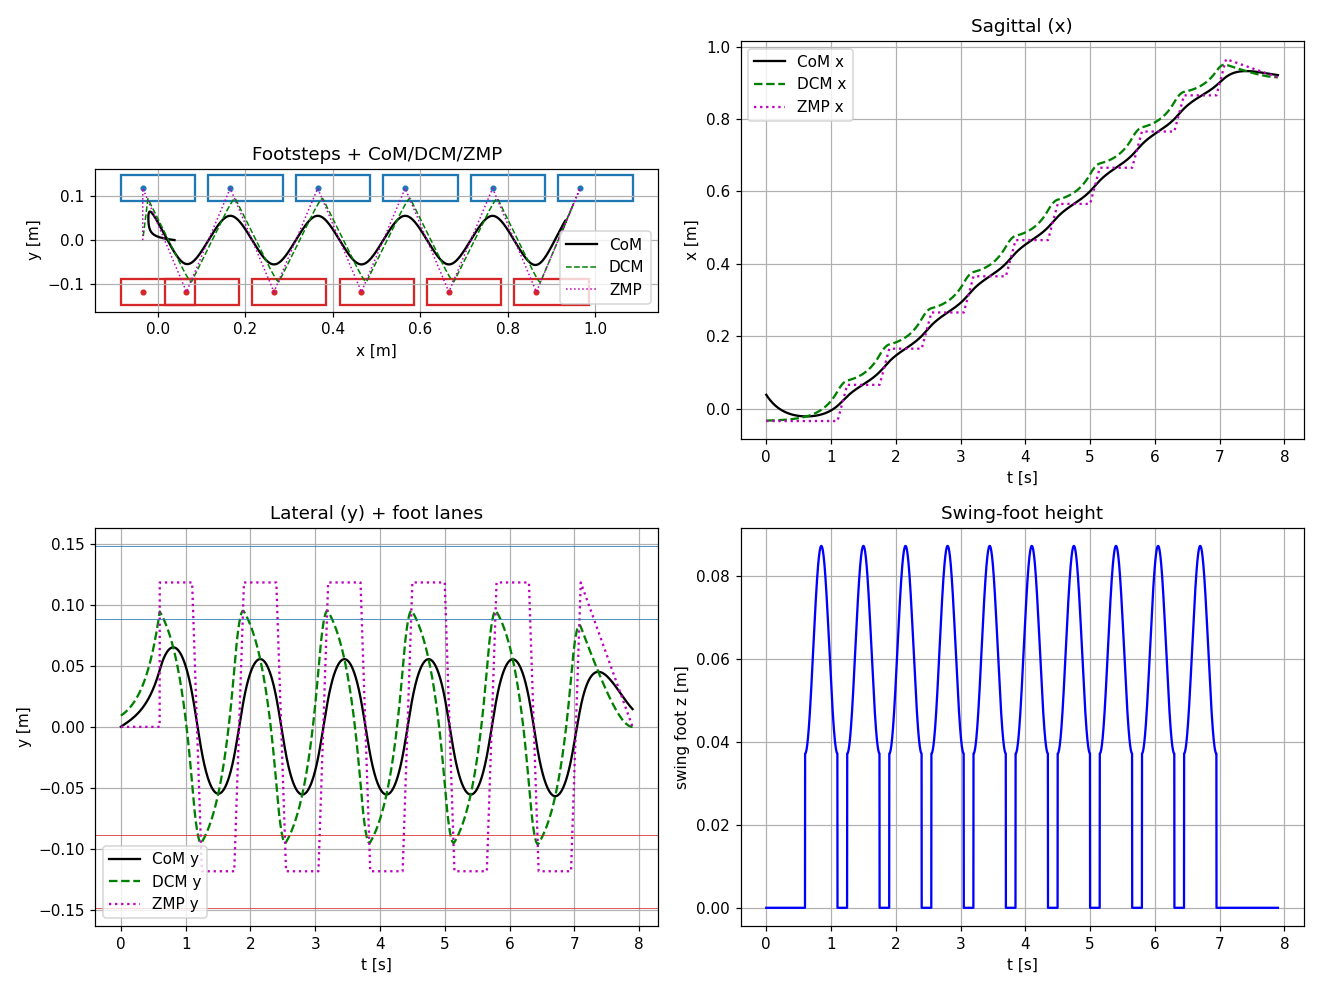
\includegraphics[width=0.85\textwidth]{stage3_plan.png}
  \caption{Offline planning output (no robot yet): footstep placement with the
  CoM, DCM and ZMP trajectories, and the swing-foot height. The ZMP steps from foot
  to foot, the DCM (capture point) leads the CoM, and the CoM weaves smoothly
  between the feet.}
  \label{fig:plan}
\end{figure}

\subsection{Terrain-aware control (flat / incline / stairs)}
\label{sec:impl:terrain}
Terrain awareness is what lets the \emph{same} controller walk on flat ground,
inclines and small stairs. A \texttt{Terrain} object (\texttt{src/planning/terrain.py})
does two jobs: it mutates the model at load time via \texttt{mjSpec} (tilting the
floor for an incline, adding stair boxes), and it exposes
$\texttt{height}(x,y)$, $\texttt{normal}(x,y)$ and a per-terrain
$\texttt{footstep\_x}$. Footsteps then land \emph{on} the surface
($z=\texttt{height}(x)$), the swing foot is oriented to the surface normal so it
lands flat, the friction cones are rotated to the surface ($R_{\text{surf}}$ from
$\texttt{normal}$), and the CoM-height reference is regulated relative to the local
ground and low-passed (which removes the vertical jerk at each stair edge). On
stairs the \texttt{footstep\_x} snaps each foot onto a tread centre so the sole
never overhangs a riser.

% ===========================================================================
\section{Results: Walking and Balance}
\label{sec:results}
All results are headless and reproducible (a single \texttt{evaluate.py} battery
reproduces them); figures are produced by the corresponding scripts. Unless noted,
numbers are for the G1.

\subsection{Gravity compensation (dynamics sanity check)}
Before any walking, we verify that the dynamics terms are correct: we solve the
static balance $S^{\top}\tau+\sum J_c^{\top}f=h$ in double support and command the
resulting feedforward torques. The robot stays upright and essentially still
(base height drift $\approx\!1.7$~mm, dynamics residual $\sim\!10^{-4}$), proving
that $M$, $h$ and the contact Jacobians are consistent (Fig.~\ref{fig:gravcomp}).

\begin{figure}[H]\centering
  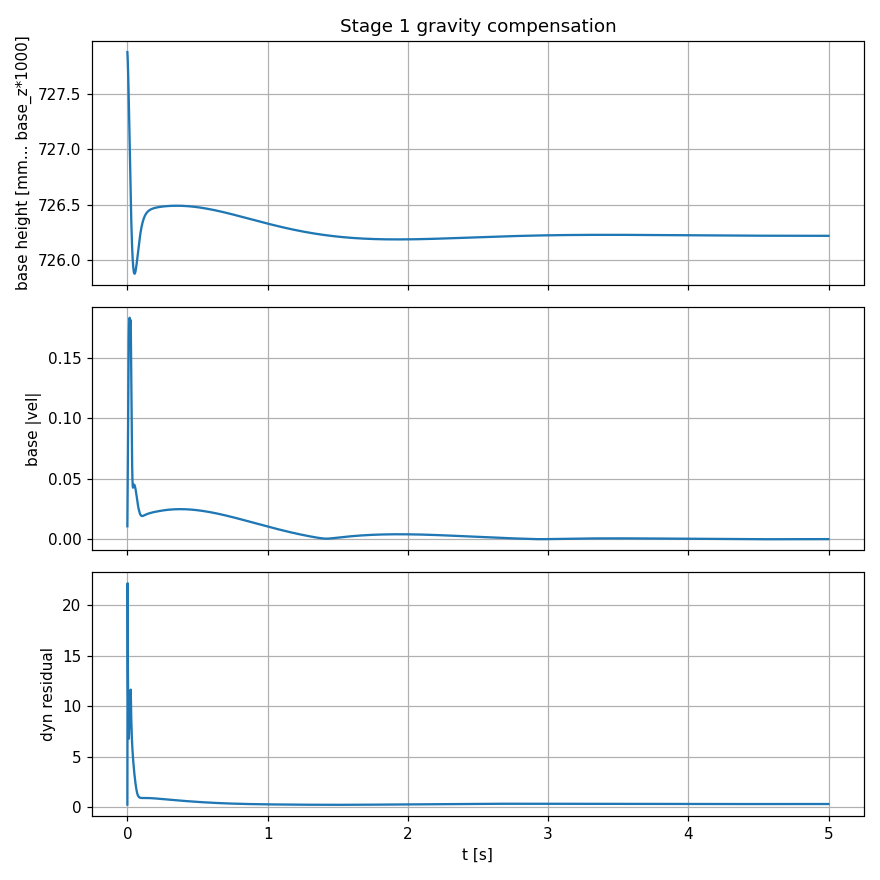
\includegraphics[width=0.7\textwidth]{stage1_gravity_comp.png}
  \caption{Gravity compensation: the robot holds its pose by feedforward torque
  alone (base height, base velocity and dynamics residual vs.\ time).}
  \label{fig:gravcomp}
\end{figure}

\subsection{Standing balance: weight shift and single support}
Driven by the whole-body QP, the robot stands stably, shifts its CoM laterally
($\pm$ several~cm), and balances on a single foot while the other is raised
(Fig.~\ref{fig:stand}). The QP is feasible at every step.

\begin{figure}[H]\centering
  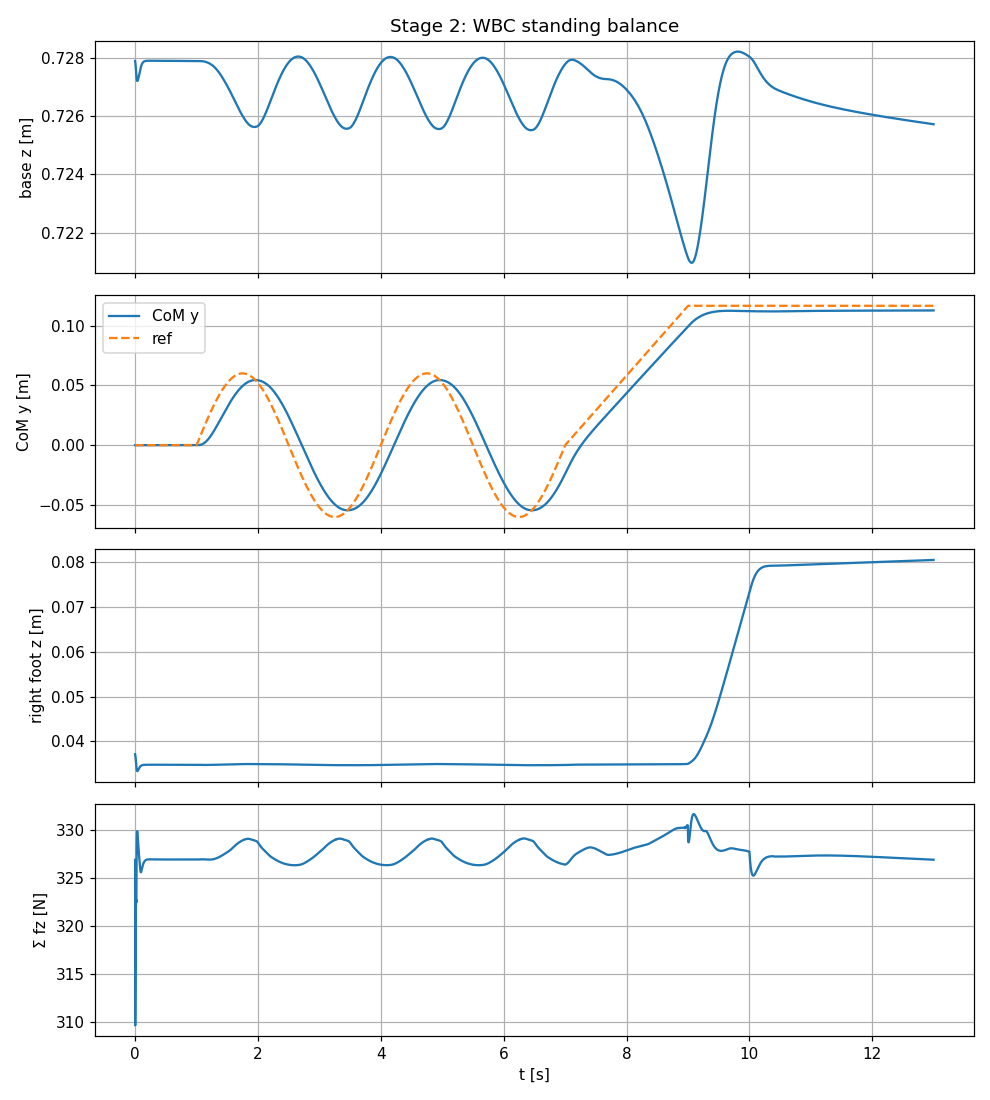
\includegraphics[width=0.75\textwidth]{stage2_stand_balance.png}
  \caption{Standing balance: base height, lateral CoM tracking during a weight
  shift, swing-foot height during single support, and total normal force.}
  \label{fig:stand}
\end{figure}

\subsection{Continuous flat walking}
With the DCM feedback and capture-point step adjustment, the G1 walks a continuous,
stable gait for the full plan ($\sim\!10$ steps, $\sim\!1$~m) without falling, with
small CoM tracking error and a pelvis tilt of only a few degrees
(Fig.~\ref{fig:flat}).

\begin{figure}[H]\centering
  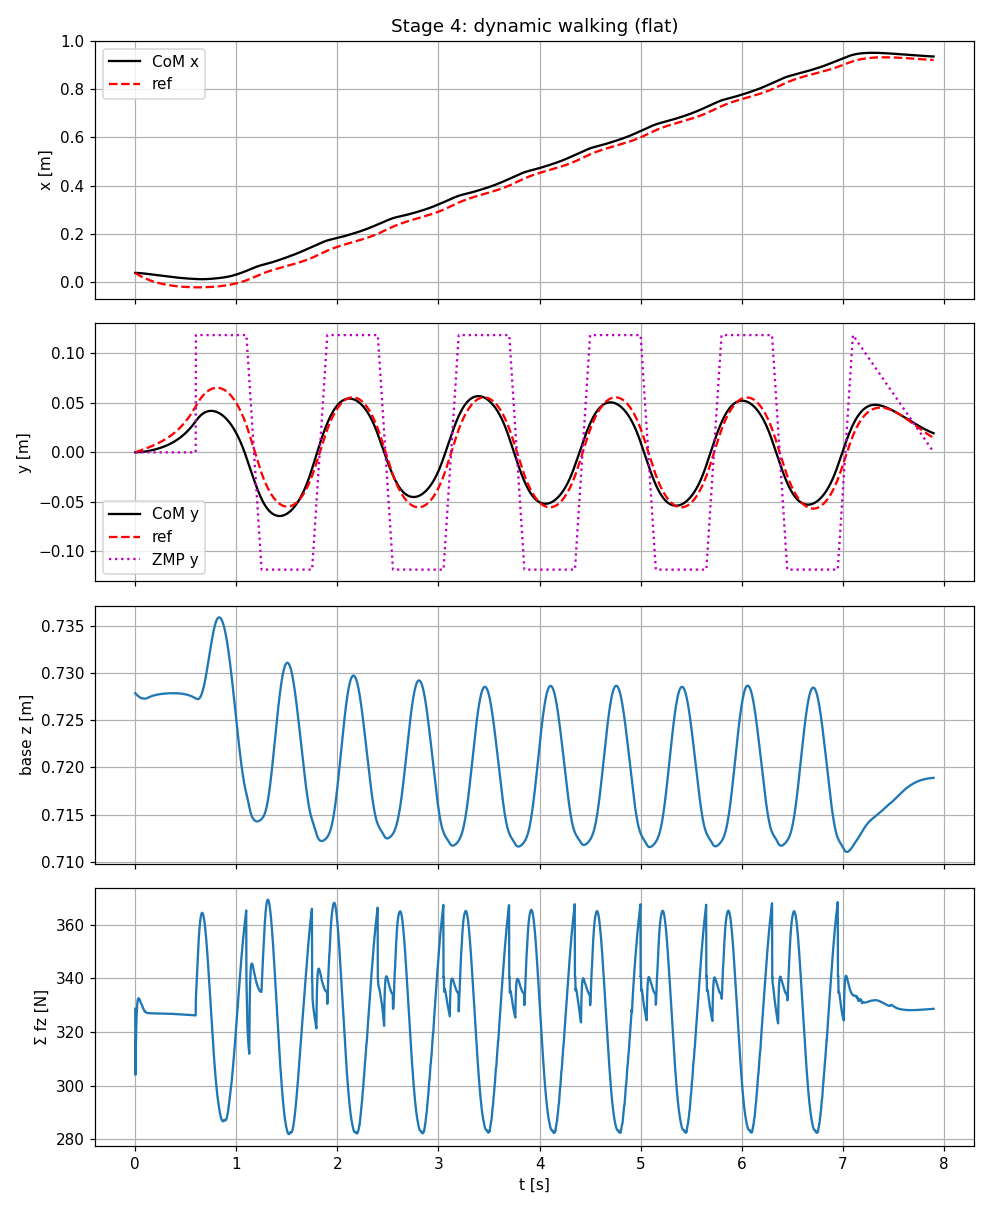
\includegraphics[width=0.8\textwidth]{stage4_walk_flat.png}
  \caption{Continuous flat walking: forward and lateral CoM vs.\ the reference,
  base height, and total contact force (the alternating SS/DS load transfer).}
  \label{fig:flat}
\end{figure}

\subsection{Inclines and stairs}
Because footsteps, friction cones and CoM height are all expressed relative to the
local surface, the same controller walks uphill and climbs small stairs. The G1
walks up inclines up to $16^{\circ}$ (Fig.~\ref{fig:incline}) and climbs a full
staircase tread-by-tread (Fig.~\ref{fig:stairs}); panel~(B) of each figure shows
the CoM height rising with the terrain.

\begin{figure}[H]\centering
  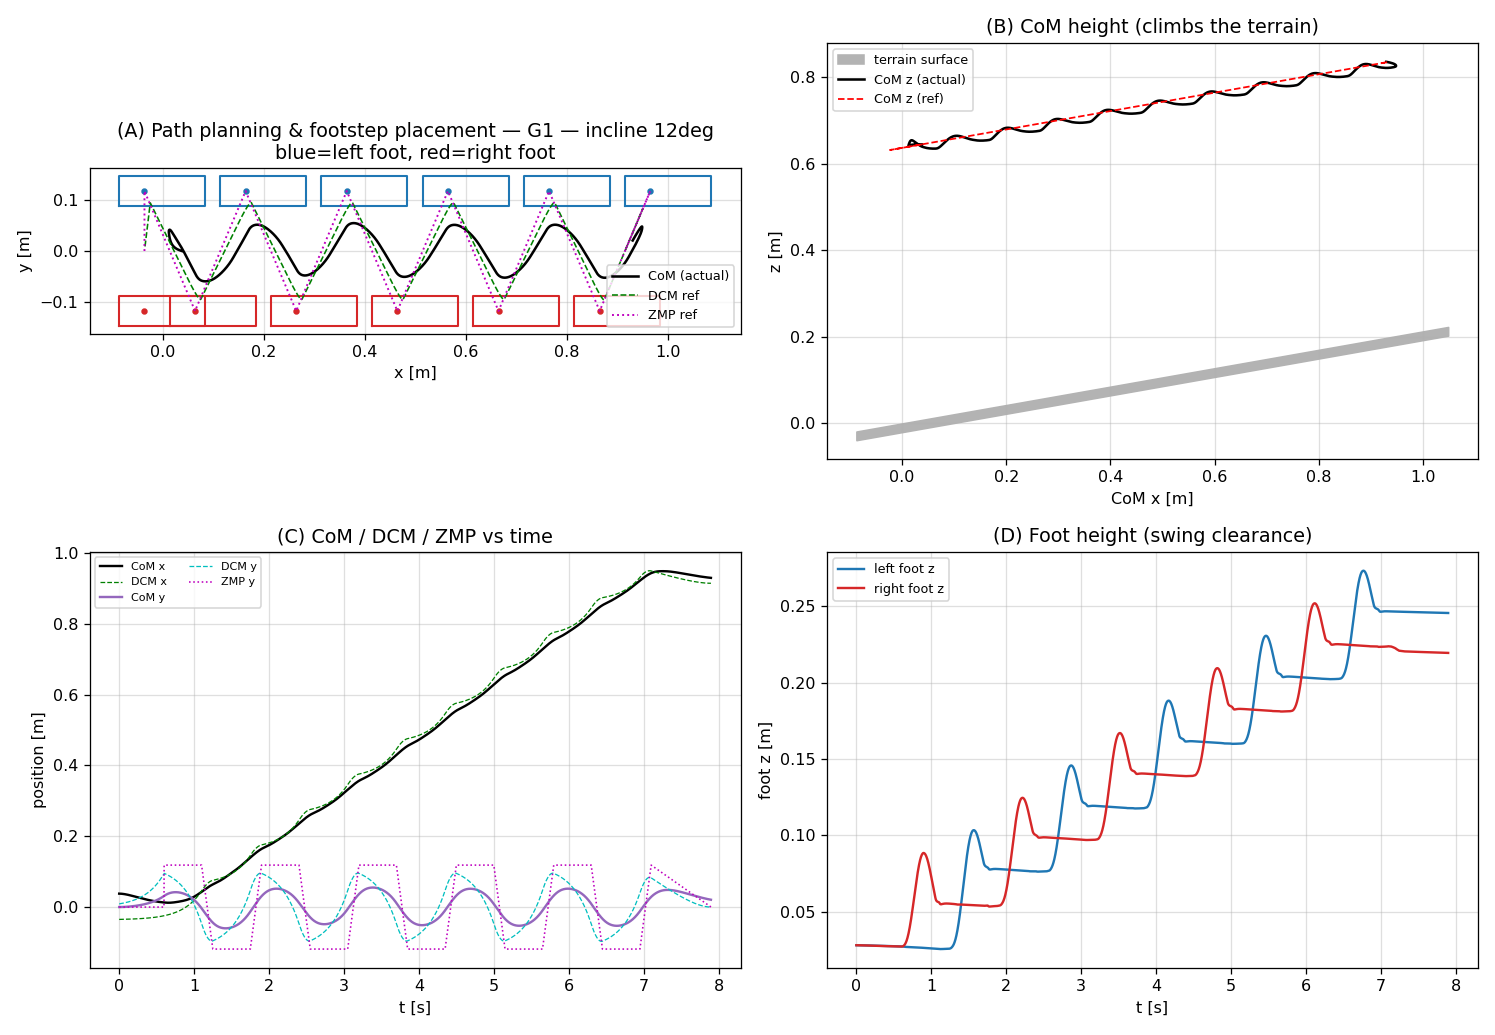
\includegraphics[width=0.92\textwidth]{plot_walk_g1_incline_12deg.png}
  \caption{Walking up a $12^{\circ}$ incline: (A) footstep placement, (B) CoM height
  climbing the slope, (C) CoM/DCM/ZMP, (D) swing-foot clearance.}
  \label{fig:incline}
\end{figure}

\begin{figure}[H]\centering
  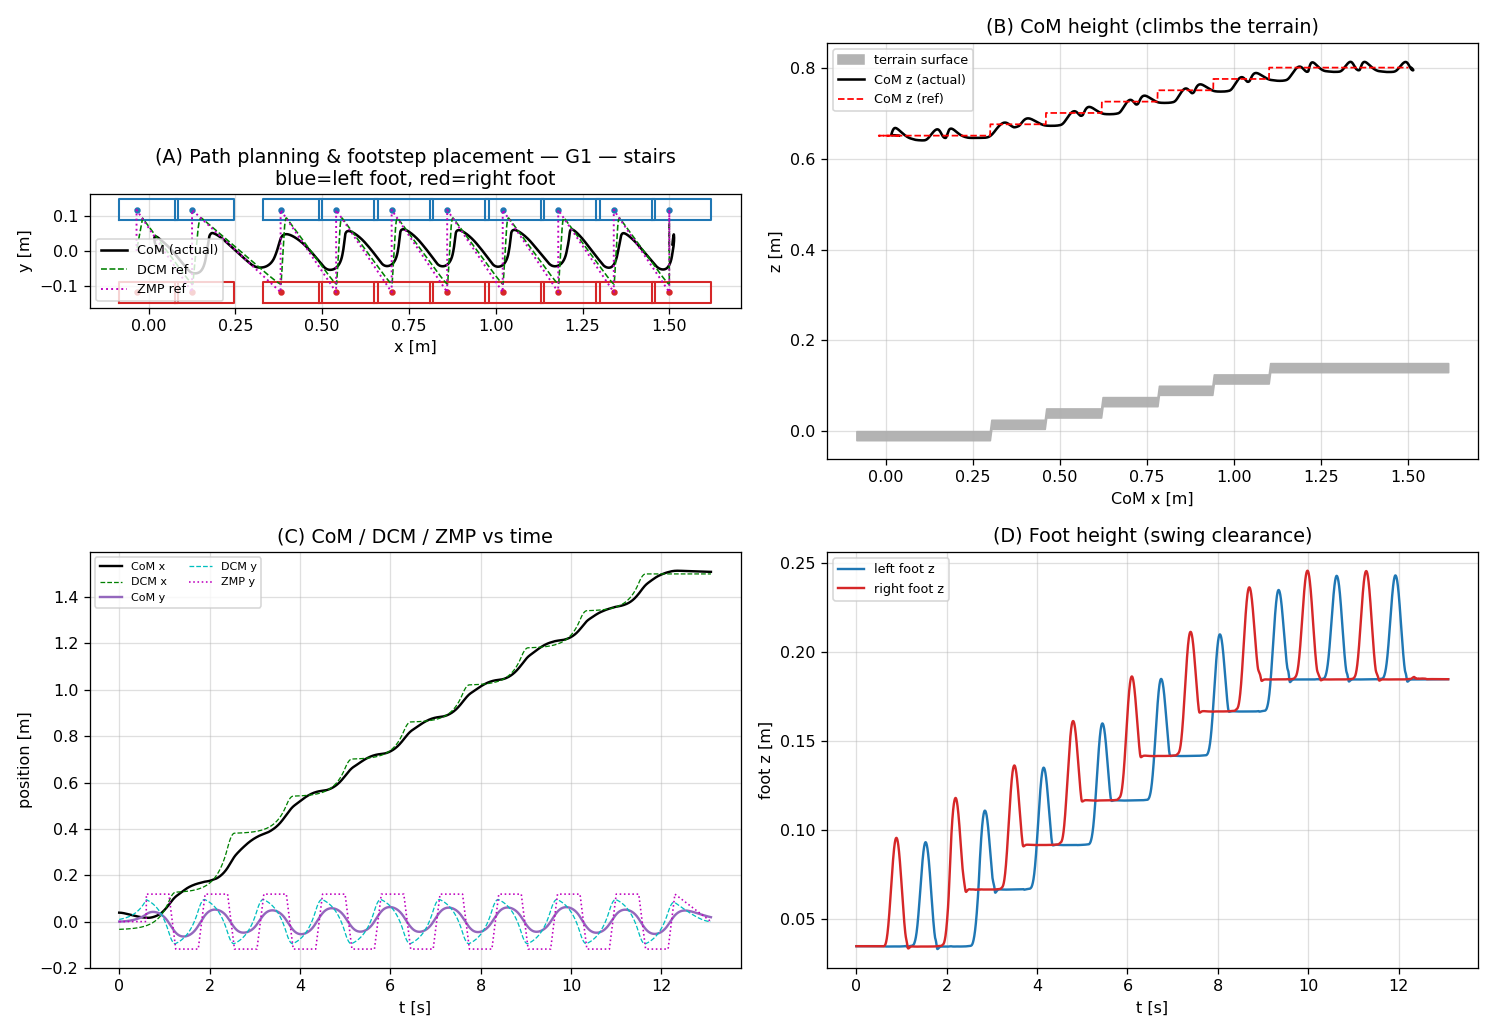
\includegraphics[width=0.92\textwidth]{plot_walk_g1_stairs.png}
  \caption{Climbing stairs (feet-together-per-tread): the CoM height (B) steps up
  with the treads; the swing foot (D) clears each riser.}
  \label{fig:stairs}
\end{figure}

\subsection{Omnidirectional walking}
The same DCM+QP stack walks in any direction from a body-frame velocity command
$(v_x,v_y,v_{\text{yaw}})$ --- forward, backward, strafing, and turning. The pelvis
yaw tracks the heading, so the robot can walk a curve (Fig.~\ref{fig:curve}).

\begin{figure}[H]\centering
  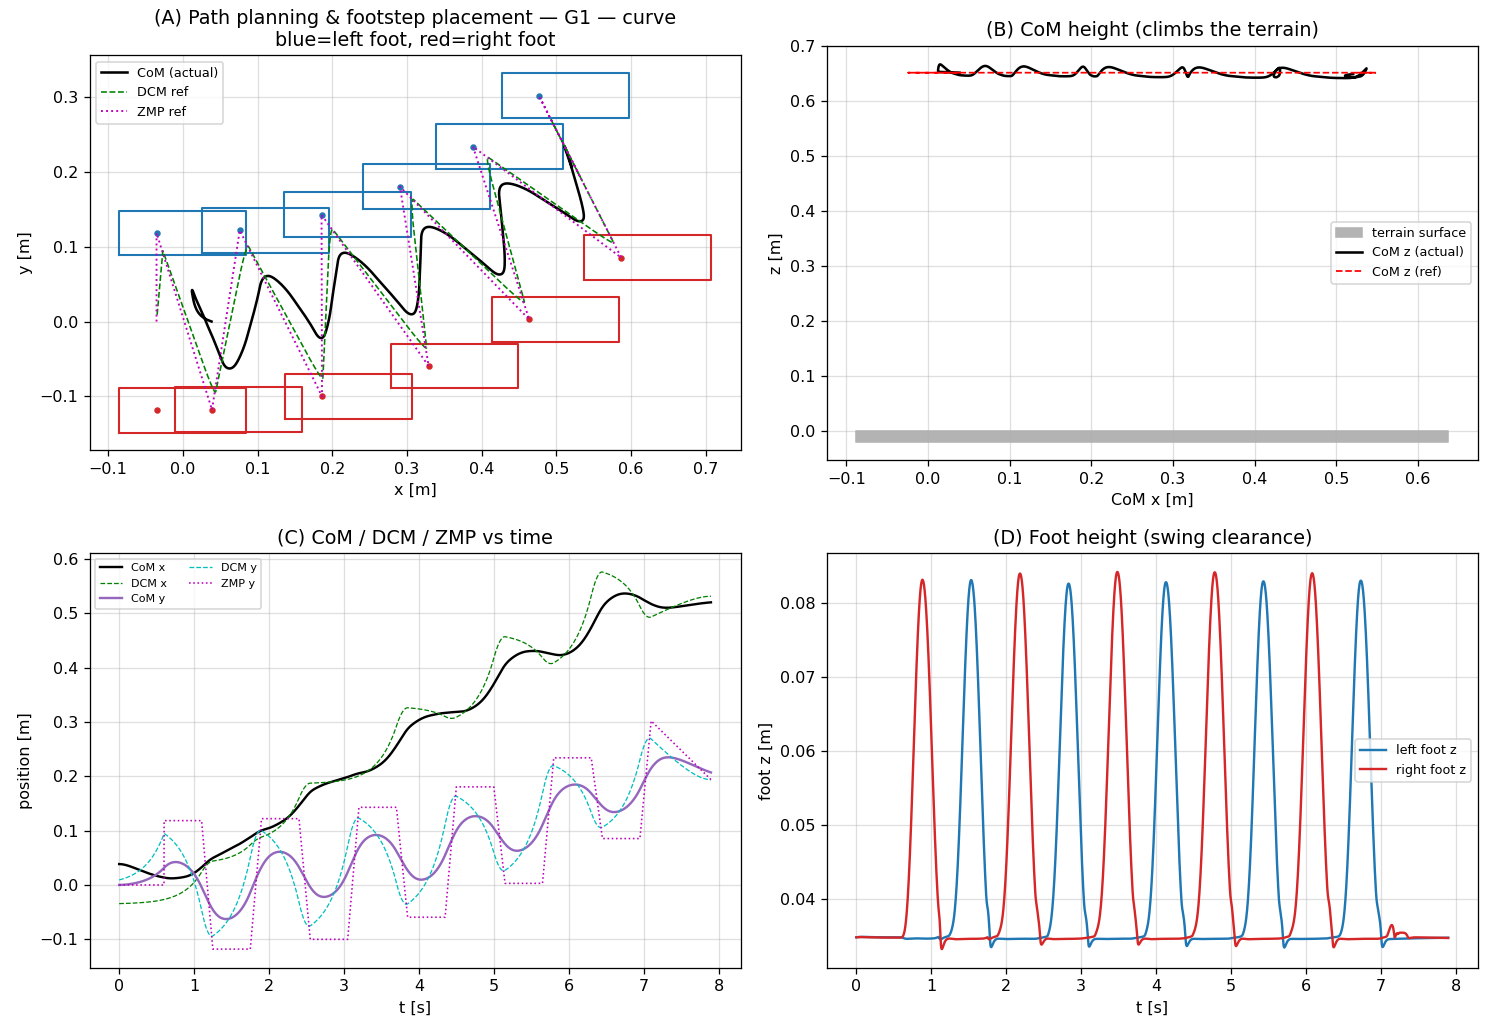
\includegraphics[width=0.92\textwidth]{plot_walk_g1_curve.png}
  \caption{Walking a curve ($v_x=0.10$, $v_{\text{yaw}}=0.12$): the footstep
  rectangles rotate with the heading and the CoM follows a curved path.}
  \label{fig:curve}
\end{figure}

\subsection{Push recovery}
While walking, external shoves are applied to the pelvis for $\sim\!100$~ms. The
capture-point step adjustment relocates the swing foot toward the perturbed DCM and
the robot recovers without falling (Fig.~\ref{fig:push}); the tolerated impulse is
larger fore--aft than laterally, reflecting the narrow foot.

\begin{figure}[H]\centering
  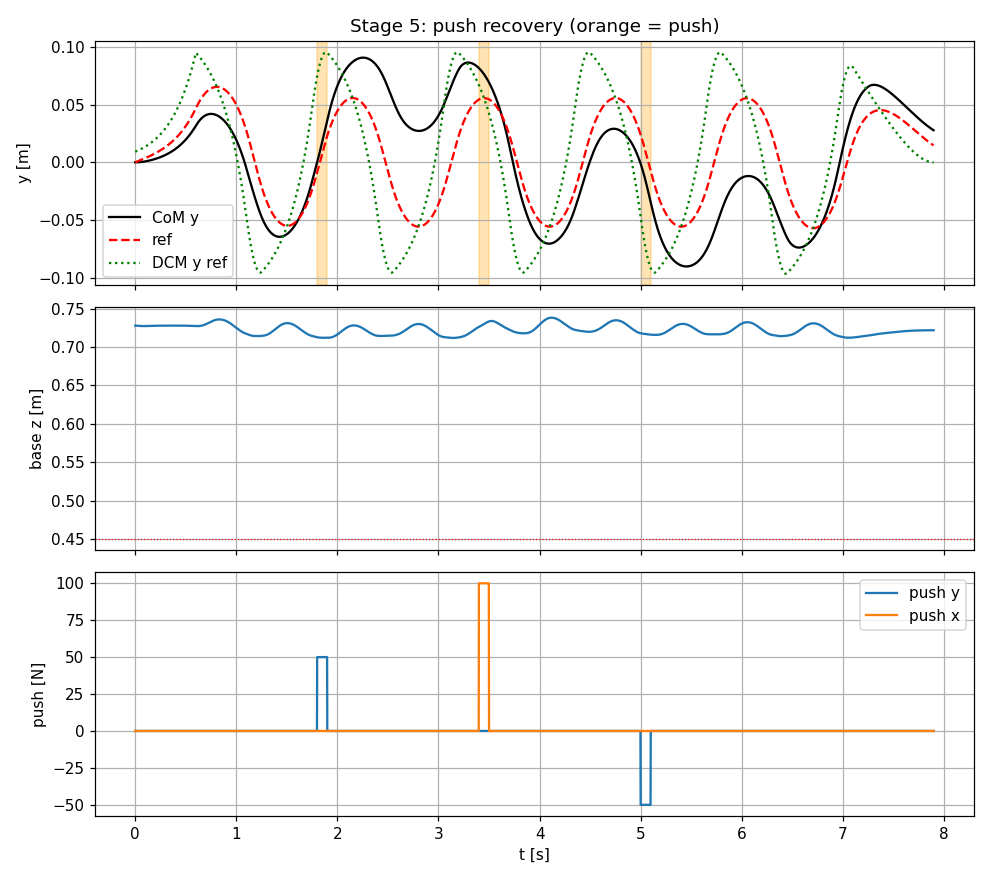
\includegraphics[width=0.8\textwidth]{stage5_push_recovery.png}
  \caption{Push recovery during walking: lateral CoM vs.\ reference (pushes shaded),
  base height, and the applied force; the robot stays upright and re-converges.}
  \label{fig:push}
\end{figure}

\subsection{Second robot: PAL Talos}
The identical controller, planner and QP run on the 94~kg Talos through its
\texttt{RobotConfig}; it stands, balances, walks on flat ground and inclines, and
recovers from pushes (Fig.~\ref{fig:talos}), demonstrating that the approach is not
tuned to a single robot.

\begin{figure}[H]\centering
  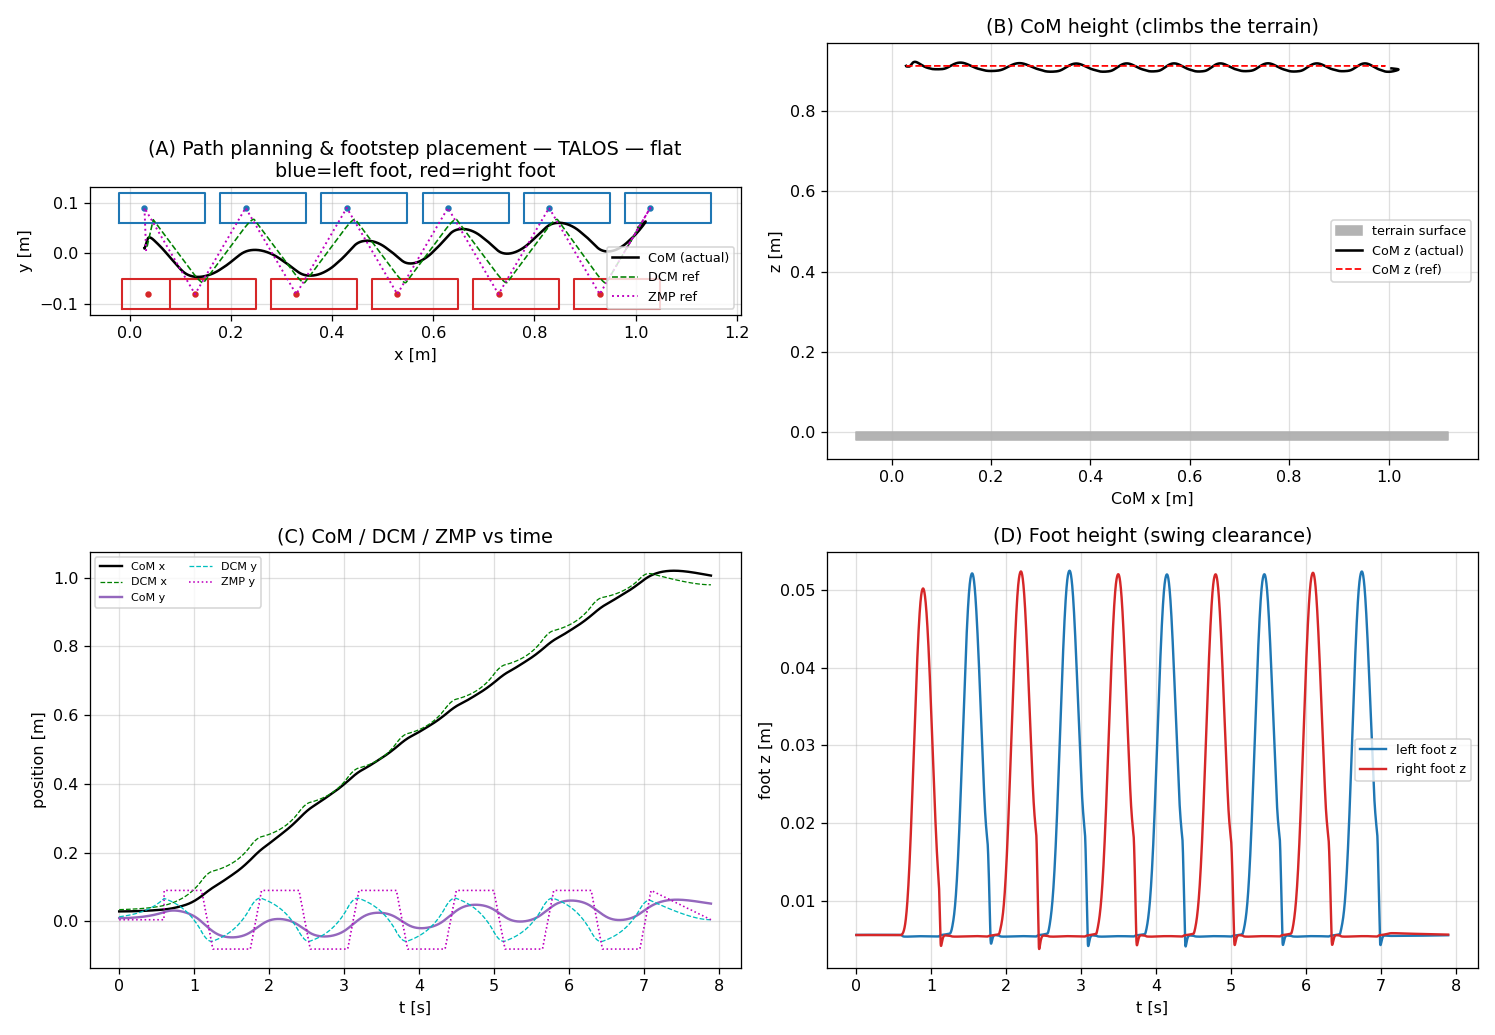
\includegraphics[width=0.8\textwidth]{plot_walk_talos_flat.png}
  \caption{PAL Talos walking on flat ground with the same controller as the G1.}
  \label{fig:talos}
\end{figure}

% ===========================================================================
\section{Incline Limit Analysis}
\label{sec:incline}
How steep a slope can the robot hold? There are two distinct failure modes, each
with a simple closed form.

\paragraph{Slipping.} The tangential component of gravity must be held by friction:
$mg\sin\alpha\le\mu\,mg\cos\alpha$, i.e.
\begin{equation}
    \alpha_{\text{slip}}=\arctan\mu .
\end{equation}
With $\mu=0.5$ this gives $\alpha_{\text{slip}}\approx 26.6^{\circ}$.

\paragraph{Tipping.} The body tips about the downhill edge of the support when the
gravity line passes outside it: $mg\cos\alpha\,d\ge mg\sin\alpha\,H$, i.e.
$\alpha_{\text{tip}}=\arctan(d/H)$, where $d$ is the horizontal distance from the
CoM to the downhill edge and $H$ the CoM height. Because the active controller
keeps the CoM well inside the support polygon, $d/H$ stays large and tipping never
binds before slipping --- so \emph{standing is slip-limited}.

\paragraph{Experiment.} Sweeping the slope angle, the robot stands stably up to
$26^{\circ}$ and slips at $27^{\circ}$, matching $\arctan\mu$ almost exactly.
Note that uphill \emph{walking} fails earlier ($\sim\!16^{\circ}$): there the limit
is dynamic (single-support balance and the unmodelled along-slope gravity in the
horizontal LIPM), not static slip or tip.

% ===========================================================================
\section{Extended Demonstrations}
\label{sec:fun}
Two integrated demos exercise the full stack (path planning $\to$ DCM $\to$ QP) on
harder, less-scripted scenarios.

\subsection{Waiter: slalom navigation around tables}
The robot is given a goal behind a field of randomly generated round tables and
must walk to it while carrying a tray with a frappe. The course is a
\emph{slalom}: tables are placed alternately left/right of the centre-line (one per
gate), and the planned trajectory is built directly as a sinusoid in
\emph{opposite phase} to the tables, so the robot threads each gate on the free
side (Fig.~\ref{fig:waiter}). The gate spacing is chosen so the sinusoid's curvature
stays within the gait's turn rate, and a walkability check resamples the (random)
layout until the path both clears every table and is gentle enough to follow. The
footstep planner places steps along this path (pelvis facing the path tangent), the
DCM+QP walk it, and the tray --- rigidly attached to the upright torso --- stays
level so the frappe does not spill (measured torso tilt $<\!6^{\circ}$).

\begin{figure}[H]\centering
  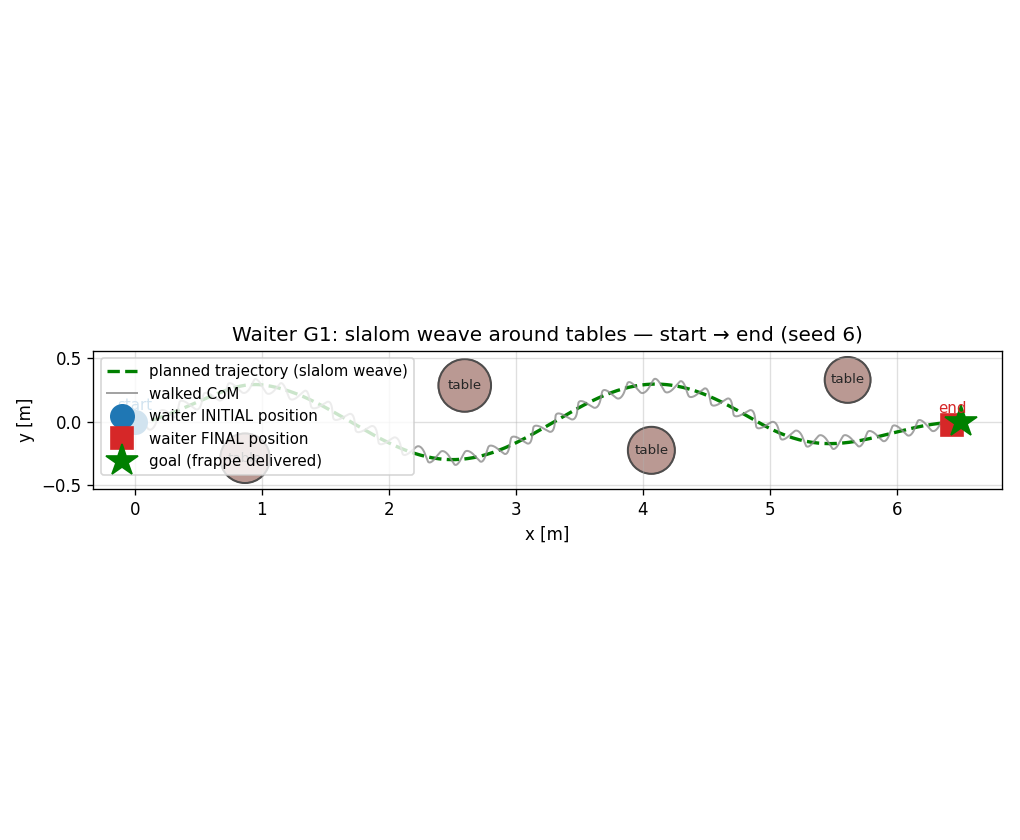
\includegraphics[width=0.78\textwidth]{navigate_waiter.png}
  \caption{Waiter task: the planned slalom trajectory weaves between randomly
  generated tables; the walked CoM follows it from the initial to the final
  position, delivering the frappe at the goal.}
  \label{fig:waiter}
\end{figure}

\subsection{Sisyphus: pushing a boulder up a slope}
The robot reaches both arms forward and pushes a large ball (at hand height,
constrained to slide along the slope) up an incline while walking uphill
(Fig.~\ref{fig:sisyphus}). A steady forward CoM bias counters the backward-tipping
torque from the high contact point --- exactly as a person leans into a push. The
ball advances in a push--rollback--push rhythm, climbing with the robot.

\begin{figure}[H]\centering
  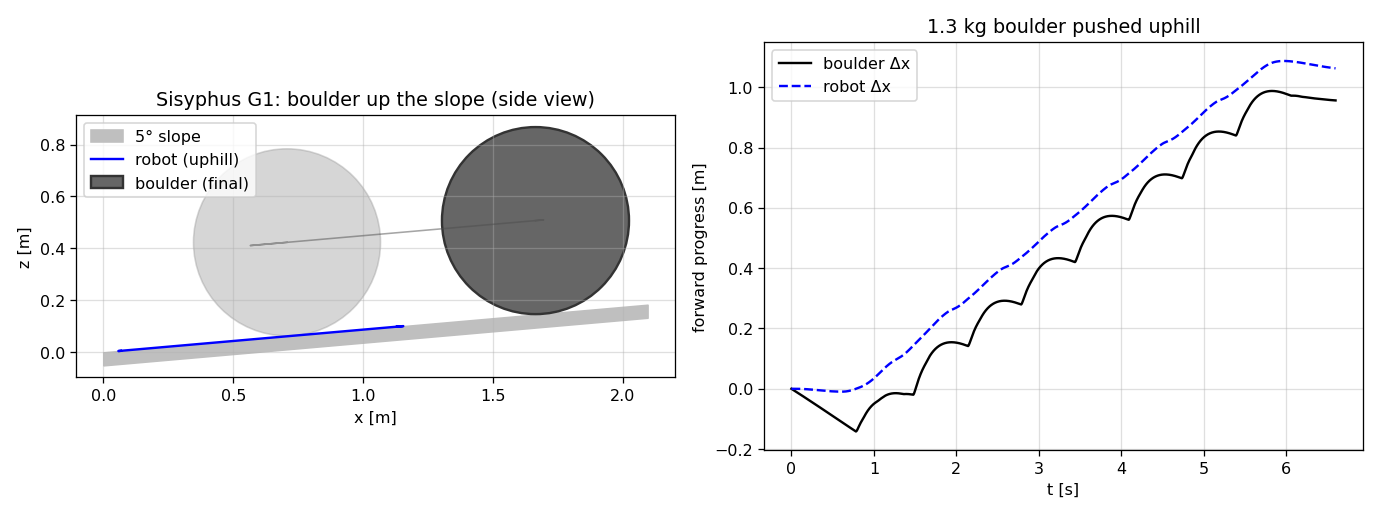
\includegraphics[width=0.92\textwidth]{sisyphus_g1_5deg.png}
  \caption{Sisyphus: (left) side view of the robot and the ball climbing the slope;
  (right) forward progress of the ball and the robot vs.\ time.}
  \label{fig:sisyphus}
\end{figure}

% ===========================================================================
\section{Parameters}
\label{sec:params}
All tunables live in \texttt{config/params.yaml}. The most important ones are
summarised in Table~\ref{tab:params}.

\begin{table}[H]\centering
\caption{Key parameters (from \texttt{config/params.yaml}).}
\label{tab:params}
\small
\begin{tabular}{@{}lll@{}}
\toprule
Parameter & Value & Meaning\\
\midrule
\multicolumn{3}{@{}l}{\textit{Whole-body QP}}\\
\quad friction $\mu$            & $0.5$         & friction coefficient (conservative)\\
\quad $f_{\min}$                & $1$~N         & min.\ normal force per contact point\\
\quad solver                   & quadprog      & dense PD solver (clarabel/osqp fallback)\\
\multicolumn{3}{@{}l}{\textit{Task weights / gains ($w$, $K_p$, $K_d$)}}\\
\quad CoM                      & $100,\,100,\,20$ & high-weight CoM task\\
\quad orientation              & $20,\,80,\,18$   & torso upright vs.\ gravity\\
\quad posture                  & $1,\,20,\,8$     & regularisation toward the crouch\\
\quad swing foot               & $120,\,300,\,34$ & airborne-foot tracking\\
\quad $k_{\text{dcm}}$         & $3.0$         & DCM feedback gain\\
\multicolumn{3}{@{}l}{\textit{Gait}}\\
\quad step length              & $0.10$--$0.20$~m & speed knob ($\approx0.11$--$0.23$~m/s)\\
\quad $t_{SS}$ / $t_{DS}$       & $0.5$ / $0.15$~s & single- / double-support duration\\
\quad swing apex               & $0.05$~m      & swing-foot peak height\\
\multicolumn{3}{@{}l}{\textit{Capture point}}\\
\quad gain / max shift         & $1.0$ / $0.12$~m & DCM-based step adjustment\\
\bottomrule
\end{tabular}
\end{table}

% ===========================================================================
\section{Discussion, Limitations and Future Work}
\label{sec:discussion}
The dynamics-first, torque-level design meets all of the assignment's core tasks:
the robot walks continuously, plans and controls its CoM, shifts its weight onto
the support foot, coordinates foot placement with body motion, stays stable through
DS$\leftrightarrow$SS transitions, and recovers from pushes and imperfect foot
placement. Expressing balance with respect to gravity and the contact surface is
what makes the controller generalise to inclines and stairs with no redesign, and
the \texttt{RobotConfig} abstraction is what lets it run on a second robot.

Several limitations remain. (i) Uphill \emph{walking} is capped near $16^{\circ}$:
the planner uses a horizontal LIPM/DCM that ignores the along-slope gravity
component; a slope-projected LIPM or an MPC formulation would push this toward the
static slip limit. (ii) Lateral push tolerance is lower than fore--aft because of
the narrow feet and the limited centre-of-pressure authority in single support;
step-\emph{timing} adaptation (landing early to catch a fall), in addition to the
current step-\emph{placement} adjustment, would help. (iii) Stair climbing is tuned
to gentle risers; taller steps need a larger step length and clearance. (iv) The QP
backend is \texttt{quadprog} rather than \texttt{proxqp} (which has no Windows
build) --- the method is identical, only the solver differs. Natural next steps are
a receding-horizon DCM/CoP MPC, an angular-momentum task for stronger push
recovery, and online navigation that re-plans the velocity command continuously.

% ===========================================================================
\section{Conclusion}
\label{sec:conclusion}
We built a torque-level, whole-body-QP walking controller for the Unitree~G1 and
PAL~Talos in MuJoCo, organised as an offline (footsteps + ZMP/DCM) $\to$ online
(DCM feedback + capture-point) $\to$ whole-body-control pipeline. The robot achieves
stable continuous walking, single-support balancing, weight shifting, push
recovery, omnidirectional walking, and locomotion over inclines and small stairs,
with a simple slip-vs-tip analysis that correctly predicts the standing limit.
Because every balance quantity is expressed with respect to gravity and the local
surface, and because the robot-specific facts are isolated in one configuration
object, the same code runs unchanged on both robots and extends naturally to the
two integrated path-planning demonstrations.

% ===========================================================================
\begin{thebibliography}{9}
\bibitem{lec9} Lecture 9, \emph{Whole-Body Control via QP}, Robotic Systems I.
\bibitem{lec10} Lecture 10, \emph{ZMP / LIPM / DCM and walking}, Robotic Systems I.
\bibitem{kuindersma} S.~Kuindersma et al., \emph{Optimization-based locomotion
  planning, estimation, and control design for Atlas}, Auton.\ Robots, 2016.
\bibitem{englsberger} J.~Englsberger et al., \emph{Three-dimensional bipedal
  walking control based on Divergent Component of Motion}, IEEE T-RO, 2015.
\bibitem{pratt} J.~Pratt et al., \emph{Capture Point: A step toward humanoid push
  recovery}, Humanoids, 2006.
\end{thebibliography}

\end{document}